% Options for packages loaded elsewhere
\PassOptionsToPackage{unicode}{hyperref}
\PassOptionsToPackage{hyphens}{url}
\PassOptionsToPackage{dvipsnames,svgnames,x11names}{xcolor}
%
\documentclass[
  10pt,
]{article}
\usepackage{amsmath,amssymb}
\usepackage{iftex}
\ifPDFTeX
  \usepackage[T1]{fontenc}
  \usepackage[utf8]{inputenc}
  \usepackage{textcomp} % provide euro and other symbols
\else % if luatex or xetex
  \usepackage{unicode-math} % this also loads fontspec
  \defaultfontfeatures{Scale=MatchLowercase}
  \defaultfontfeatures[\rmfamily]{Ligatures=TeX,Scale=1}
\fi
\usepackage{lmodern}
\ifPDFTeX\else
  % xetex/luatex font selection
\fi
% Use upquote if available, for straight quotes in verbatim environments
\IfFileExists{upquote.sty}{\usepackage{upquote}}{}
\IfFileExists{microtype.sty}{% use microtype if available
  \usepackage[]{microtype}
  \UseMicrotypeSet[protrusion]{basicmath} % disable protrusion for tt fonts
}{}
\makeatletter
\@ifundefined{KOMAClassName}{% if non-KOMA class
  \IfFileExists{parskip.sty}{%
    \usepackage{parskip}
  }{% else
    \setlength{\parindent}{0pt}
    \setlength{\parskip}{6pt plus 2pt minus 1pt}}
}{% if KOMA class
  \KOMAoptions{parskip=half}}
\makeatother
\usepackage{xcolor}
\usepackage[margin=22mm]{geometry}
\usepackage{graphicx}
\makeatletter
\def\maxwidth{\ifdim\Gin@nat@width>\linewidth\linewidth\else\Gin@nat@width\fi}
\def\maxheight{\ifdim\Gin@nat@height>\textheight\textheight\else\Gin@nat@height\fi}
\makeatother
% Scale images if necessary, so that they will not overflow the page
% margins by default, and it is still possible to overwrite the defaults
% using explicit options in \includegraphics[width, height, ...]{}
\setkeys{Gin}{width=\maxwidth,height=\maxheight,keepaspectratio}
% Set default figure placement to htbp
\makeatletter
\def\fps@figure{htbp}
\makeatother
\setlength{\emergencystretch}{3em} % prevent overfull lines
\providecommand{\tightlist}{%
  \setlength{\itemsep}{0pt}\setlength{\parskip}{0pt}}
\setcounter{secnumdepth}{-\maxdimen} % remove section numbering
\ifLuaTeX
  \usepackage{selnolig}  % disable illegal ligatures
\fi
\usepackage{bookmark}
\IfFileExists{xurl.sty}{\usepackage{xurl}}{} % add URL line breaks if available
\urlstyle{same}
\hypersetup{
  colorlinks=true,
  linkcolor={Maroon},
  filecolor={Maroon},
  citecolor={Blue},
  urlcolor={blue},
  pdfcreator={LaTeX via pandoc}}

\author{}
\date{}

\begin{document}

\section{APS next leads --- 2026-11-05}\label{aps-next-leads-2026-11-05}

This search proposes four follow-ups to the merged APS implementation: a
nonhorizontal line chart, APS-specific F4 trace reuse, incremental
factor-base frontiers, and unequal partition profiles. They are
hypotheses, with explicit correctness and cost rejection criteria. None
has an APS implementation or a performance result in this study
{[}pcc:unverified{]}.

Producer proposal record:
\href{../../pcc/claims/PCC-20261105-aca921.json}{PCC-20261105-aca921}.
Identity-record assertion:
\href{../../pcc/claims/PCC-20261105-ac1e93.json}{PCC-20261105-ac1e93}.
Both have unverified standing. The public change does not include the
private native ledger additions or promote either assertion.

Deliverables: this report, \href{SOURCES.md}{source review},
\href{leads.dot}{editable diagram}, \href{leads.svg}{vector diagram},
\href{report.pdf}{report PDF}, and \href{CHECKS.md}{validation scope}.

\begin{figure}
\centering
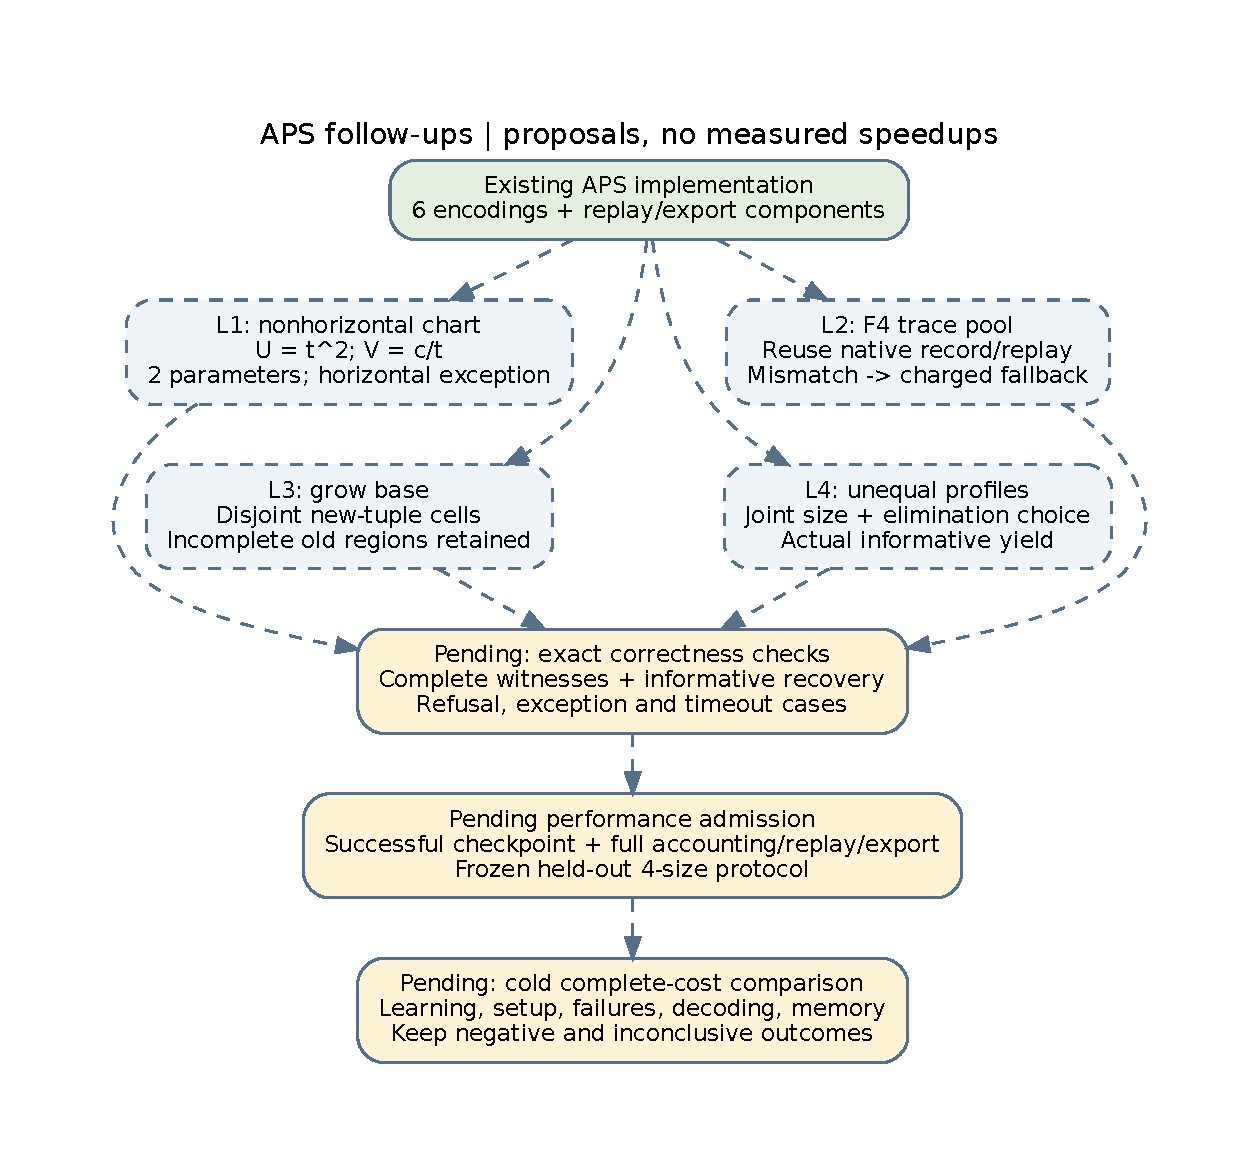
\includegraphics{leads.pdf}
\caption{Proposed APS follow-ups and their admission checks}
\end{figure}

\subsection{Scope and method}\label{scope-and-method}

Read the existing APS studies and lead register before the primary
literature, then compare the proposals with the current solver and
adapter. The source snapshot is main
\texttt{2d33e9c068c0f2b3226893017c8ea48548cc0749}. The APS, F4, native
identity-checker and SHA-256 files used here match that snapshot's
blobs; exact pins are in SOURCES.md {[}pcc:unverified{]}.

The mathematical domain is a nonsingular short Weierstrass curve
\(E: y^2=x^3+ax+b\) over \(\mathbb F_p\), \(p>3\), with labeled points
in an odd prime-order subgroup. Coordinates in the base are distinct,
and their ordinates are nonzero. No new curve instance, ECDLP run,
target set or seed population was selected. The identity-record field
below is a checker field, not an experimental ECDLP instance.

The review is bounded. In particular, Kudo et al.'s CANS 2018 full text
remains unavailable. These are proposed extensions of this
implementation, without a claim of global novelty.

\subsection{L1 --- remove the inverse variable from the pruned line
chart}\label{l1-remove-the-inverse-variable-from-the-pruned-line-chart}

\textbf{Priority: first algebraic implementation.} The current
certified-pruned line builder has parameters \((t,c,z)\), including
\(tz-1=0\). The ordinary line encoding is already implemented; this
proposal changes its chart {[}pcc:unverified{]}.

For a nonhorizontal line \(y=tx+c\), propose

\[U=t^2,\qquad V=c/t,\qquad
H_{U,V}(X)=X^3-U(X+V)^2+aX+b.\]

Require \(H_{U,V}\mid F_{\mathcal V}\), where
\(F_{\mathcal V}(X)=\prod_{x\in\mathcal V}(X-x)\) is the squarefree base
polynomial. This uses two solver parameters and identifies the global
sign pair \((t,c)\) and \((-t,-c)\) {[}pcc:unverified{]}.

The conditional lifting argument is the useful part. If a solution of
this divisibility system had \(U=0\), every root of its cubic would have
ordinate zero, contradicting the base assumption. At any root \(x\) of a
valid cubic, the known lift satisfies \(y_x^2=U(x+V)^2\). Since
\(y_x\ne0\), also \(x+V\ne0\); thus \(U\) is a nonzero square and
\(t=y_x/(x+V)\), \(c=tV\) recovers a line. Conversely, substituting a
nonzero slope yields the displayed cubic. This is a producer derivation;
scheme-level behavior and the implementation are not independently
proved {[}pcc:unverified{]}.

\textbf{Exceptional cases.} Horizontal lines are outside this chart.
Omit them only when the existing orbit-and-label certificate establishes
that their relations are uninformative; otherwise retain a separate
horizontal chart. Reject ordinate-zero inputs and keep all base and
subgroup checks. A square root, or the point-based division above, still
costs work. Cubic terms such as \(UV^2\) may make elimination worse
despite the smaller variable count.

\textbf{First check and rejection rule.} Implement behind a separate
encoding choice. Compare complete coordinate-witness and
informative-recovery sets against the existing pruned encoding and
exhaustive tiny-field oracle; cover missing chart, zero-ordinate,
repeated-root and refusal cases. Then compare the full cold pipeline
including decoding. Reject any mismatch; retire the optimization if
degree or matrix growth erases the cost saving.

The substitution expansion has record
\href{certificates/line-chart.json}{IDC1h9e131e5cd24a395f}. This record
evaluates a polynomial identity over \(2^{61}-1\); it does not certify
the lifting argument, all prime fields, or an algorithmic benefit
{[}pcc:unverified{]}.

\subsection{L2 --- reuse F4 traces across attempts within one APS
solve}\label{l2-reuse-f4-traces-across-attempts-within-one-aps-solve}

\textbf{Priority: first solver integration.} The core already implements
\texttt{f4\_record}, \texttt{f4\_replay} and \texttt{trace\_mismatch};
APS currently does not call the tracing functions. Binary
\texttt{polynomial\_reuse} is also prior code. The new work is the
prime-field APS orchestration {[}pcc:unverified{]}.

Maintain a bounded trace pool keyed by field, encoding, partition-size
profile, variable order and input leading monomials. Learn on one
attempt and replay on later attempts with the same target. Candidate
clustering keys may also include a degree or staircase fingerprint; they
must not require the answer or uncharged pre-solving. A leading-monomial
match is necessary evidence, not a proof of a complete output basis.

Reject mismatched or uncertified replays, fall back to ordinary F4, and
charge both paths. Independently validate complete basis/root coverage
when claiming exhaustion; finding one verified witness does not certify
that a replay found every root. Preserve first-informative termination
and account for batches that continue after the first answer
{[}pcc:unverified{]}.

Demin's July 2026 Groebner.jl paper exposes learn/apply and batched
tracing on other polynomial families. It supports this implementation
direction, but its timings and break-even counts are not APS
measurements.

\textbf{First check and rejection rule.} Replay exact systems against
ordinary F4 and the existing independent replayer, including nongeneric
coefficient specializations and deliberate mismatch controls. A
subsequent cost panel must include learning, failed replay, fallback,
cache memory and speculative batch work. Judge amortization within a
single target's actual attempts. Drop this route if cold learning is not
recovered at that horizon.

\subsection{L3 --- grow a labeled base and search only newly admitted
tuples}\label{l3-grow-a-labeled-base-and-search-only-newly-admitted-tuples}

\textbf{Priority: after complete-coverage bookkeeping.} APS normally
replaces an unsuitable base. Propose retaining it, adding independent
labeled samples, and searching the new tuple frontier
{[}pcc:unverified{]}.

For disjoint increments \(\Delta_i\) and \(T_i=S_i\cup\Delta_i\), the
proposed disjoint cover is

\[\left(\prod_i T_i\right)\setminus\left(\prod_i S_i\right)
=\bigsqcup_{j=1}^{m}
\left(\prod_{i<j}S_i\right)\times\Delta_j\times
\left(\prod_{i>j}T_i\right).\]

A tuple's first new coordinate chooses its unique cell. With singleton
increments each cell fixes one coordinate, creating smaller hybrid
problems. The three-part cardinality expansion is recorded as
\href{certificates/frontier-count.json}{IDC1ha14548fc2b5ce5c3}; the set
argument is producer prose {[}pcc:unverified{]}.

\textbf{The trap:} a larger coordinate set weakens the membership
constraint. Appending the old membership equations would exclude new
solutions. Use the disjoint frontier, rather than assuming an old
Gröbner basis can be extended by adding equations. Skip the old region
only after a complete no-informative-witness result; a timeout or
partial stream is not such a certificate. Preserve incomplete regions
for later coverage.

\textbf{First check and rejection rule.} Check that old coverage plus
the frontier equals a fresh full-base search, including signed
recoveries and partially completed stages. Preserve the sampler's
conditional law and count sampling, all unsuccessful stages, saved
coverage and memory. Compare against both discard-and-resample and
one-shot construction of the final base; use an incremental group-join
control. Reject any coverage gap and abandon growth if unsuccessful
early stages cost more than the work retained.

\subsection{L4 --- optimize unequal partition sizes together with
elimination}\label{l4-optimize-unequal-partition-sizes-together-with-elimination}

\textbf{Priority: a small, interpretable protocol extension.} The
sampler already accepts a size vector; the public adapter exposes a
single \texttt{subset\_size}. Add an explicit profile and select the
guessed variable jointly with it. Hybrid solving itself is existing work
{[}pcc:unverified{]}.

At fixed total base size nine, profiles \((3,3,3)\) and \((1,4,4)\)
admit 27 and 16 coordinate tuples, respectively. The latter fixes one
variable. Under a rare-event model with yield proportional to the
product of part sizes, its whole-attempt cost would need to fall below
\(16/27\) of the balanced cost to improve expected effort. This ratio is
a heuristic break-even illustration, not an exact relation-probability
claim {[}pcc:unverified{]}.

Use fixed total distinct points and a frozen set of profiles, variable
orders and hybrid choices. Repartition identical labeled points when the
label scheme permits it; do not silently change coefficients or
informative-yield populations. A setup-cost floor can defeat the trade
even if solving becomes very cheap.

\textbf{First check and rejection rule.} Extend exact-domain replay to
unequal profiles and compare with exhaustive signed enumeration. Then
record actual informative yield and full cold cost, with held-out
profiles/instances. Keep the balanced profile as the control. Stop
profiles whose measured yield loss exceeds their cost reduction; select
on training data and evaluate the frozen choice on held-out data.

\subsection{Ideas screened out and remaining
dependencies}\label{ideas-screened-out-and-remaining-dependencies}

Fixed guaranteed label weights and their precomputed shifts are already
implemented. Multiplicative cosets and composed low-degree
rational/isogeny maps are established prior work {[}pcc:unverified{]}.
No new encoding credit is assigned to the invariants \((t^2,tc,c^2)\)
without establishing a useful delta from the existing unordered cubic
representation.

No new experiment, performance/EKS session or timing panel ran. The
source checkpoint still needs secure authentication, and complete
accounting, native replay/export coverage, frozen held-out four-size
protocol and run admission remain prerequisites to any performance
launch. Their completion is separate from this planning deliverable
{[}pcc:unverified{]}.

The index-calculus scoreboard and progress timeline remain unchanged:
this round adds proposed mechanisms and algebra records, not a new
verified edge, curve or measured value. Existing frozen studies and
receipts are preserved {[}pcc:unverified{]}.

\subsection{Execution checklist}\label{execution-checklist}

\begin{itemize}
\tightlist
\item[$\boxtimes$]
  Review repository work and primary sources; record the full-text gap.
\item[$\boxtimes$]
  Specify four distinct deltas, assumptions and rejection criteria.
\item[$\boxtimes$]
  Ship native identity records, replay receipt, diagram and inspected
  PDF.
\item[$\square$]
  Independently establish the chart and frontier completeness claims.
\item[$\square$]
  Implement each lead in a separately scoped follow-up with correctness
  checks.
\item[$\square$]
  Satisfy checkpoint and frozen-protocol prerequisites before cost
  experiments.
\item[$\square$]
  Measure held-out complete costs; retain nulls, failures and timeouts.
\end{itemize}

Planning completion does not complete T9 or the complete-cost research
panel.

\subsection{Primary references}\label{primary-references}

\begin{enumerate}
\def\labelenumi{\arabic{enumi}.}
\tightlist
\item
  Amadori, Pintore, Sala, \emph{On the discrete logarithm problem for
  prime-field elliptic curves}, revised manuscript (2018), §§3.1--3.2.
  \url{https://eprint.iacr.org/2017/609}. Author copy and checked
  sections: SOURCES.md.
\item
  Demin, \emph{Groebner.jl: Fast Gröbner Tracing in Julia} (2026),
  §§2--4. \url{https://arxiv.org/html/2607.06372v1}.
\item
  Milne, \emph{Elliptic Curves}, second edition, §I.3, for the chord law
  and ordinate-zero two-torsion exception.
  \url{https://www.jmilne.org/math/Books/EC2.pdf}.
\item
  Petit, Kosters, Messeng, \emph{Algebraic approaches for the Elliptic
  Curve Discrete Logarithm Problem over prime fields} (PKC 2016).
  \url{https://christophe.petit.web.ulb.be/files/16PKC_primeECDLP.pdf}.
\item
  Kudo et al., \emph{Acceleration of Index Calculus for Solving ECDLP
  over Prime Fields and Its Limitation} (CANS 2018);
  bibliography/abstract only.
  \url{https://doi.org/10.1007/978-3-030-00434-7_19}.
\end{enumerate}

\subsection{PCC attachment correction}\label{pcc-attachment-correction}

The original PCC records attached \texttt{identity.certificate/v1}
artifacts using PCC's \texttt{certificate} type, whose contract requires
\texttt{pcc.solve-certificate/v1}. The PCC gate correctly rejected that
mismatch. The current records retain the same statements, scopes and
artifact pins as unsigned \texttt{attestation} subjects; they remain
unverified and the native verifier reports \texttt{not\_covered}.
Byte-identical historical records, the failed check, and the old-to-new
map are retained in \url{CORRECTION.md}. No polynomial identity,
research assertion, verifier or test assertion changed
{[}pcc:unverified{]}.

\end{document}
